\documentclass{article}

\usepackage{graphicx}
\usepackage{tikz}
\usepackage{tikzsymbols}
\usetikzlibrary{calc,patterns,shapes.geometric}
\pagestyle{empty}
\usepackage[margin=0pt]{geometry}
\geometry{papersize={14in,12in}}

\def\centerarc[#1](#2)(#3:#4:#5){\draw[#1] ($(#2)+({#5*cos(#3)},{#5*sin(#3)})$) arc (#3:#4:#5);}

\begin{document}
	\begin{figure}
		\centering
		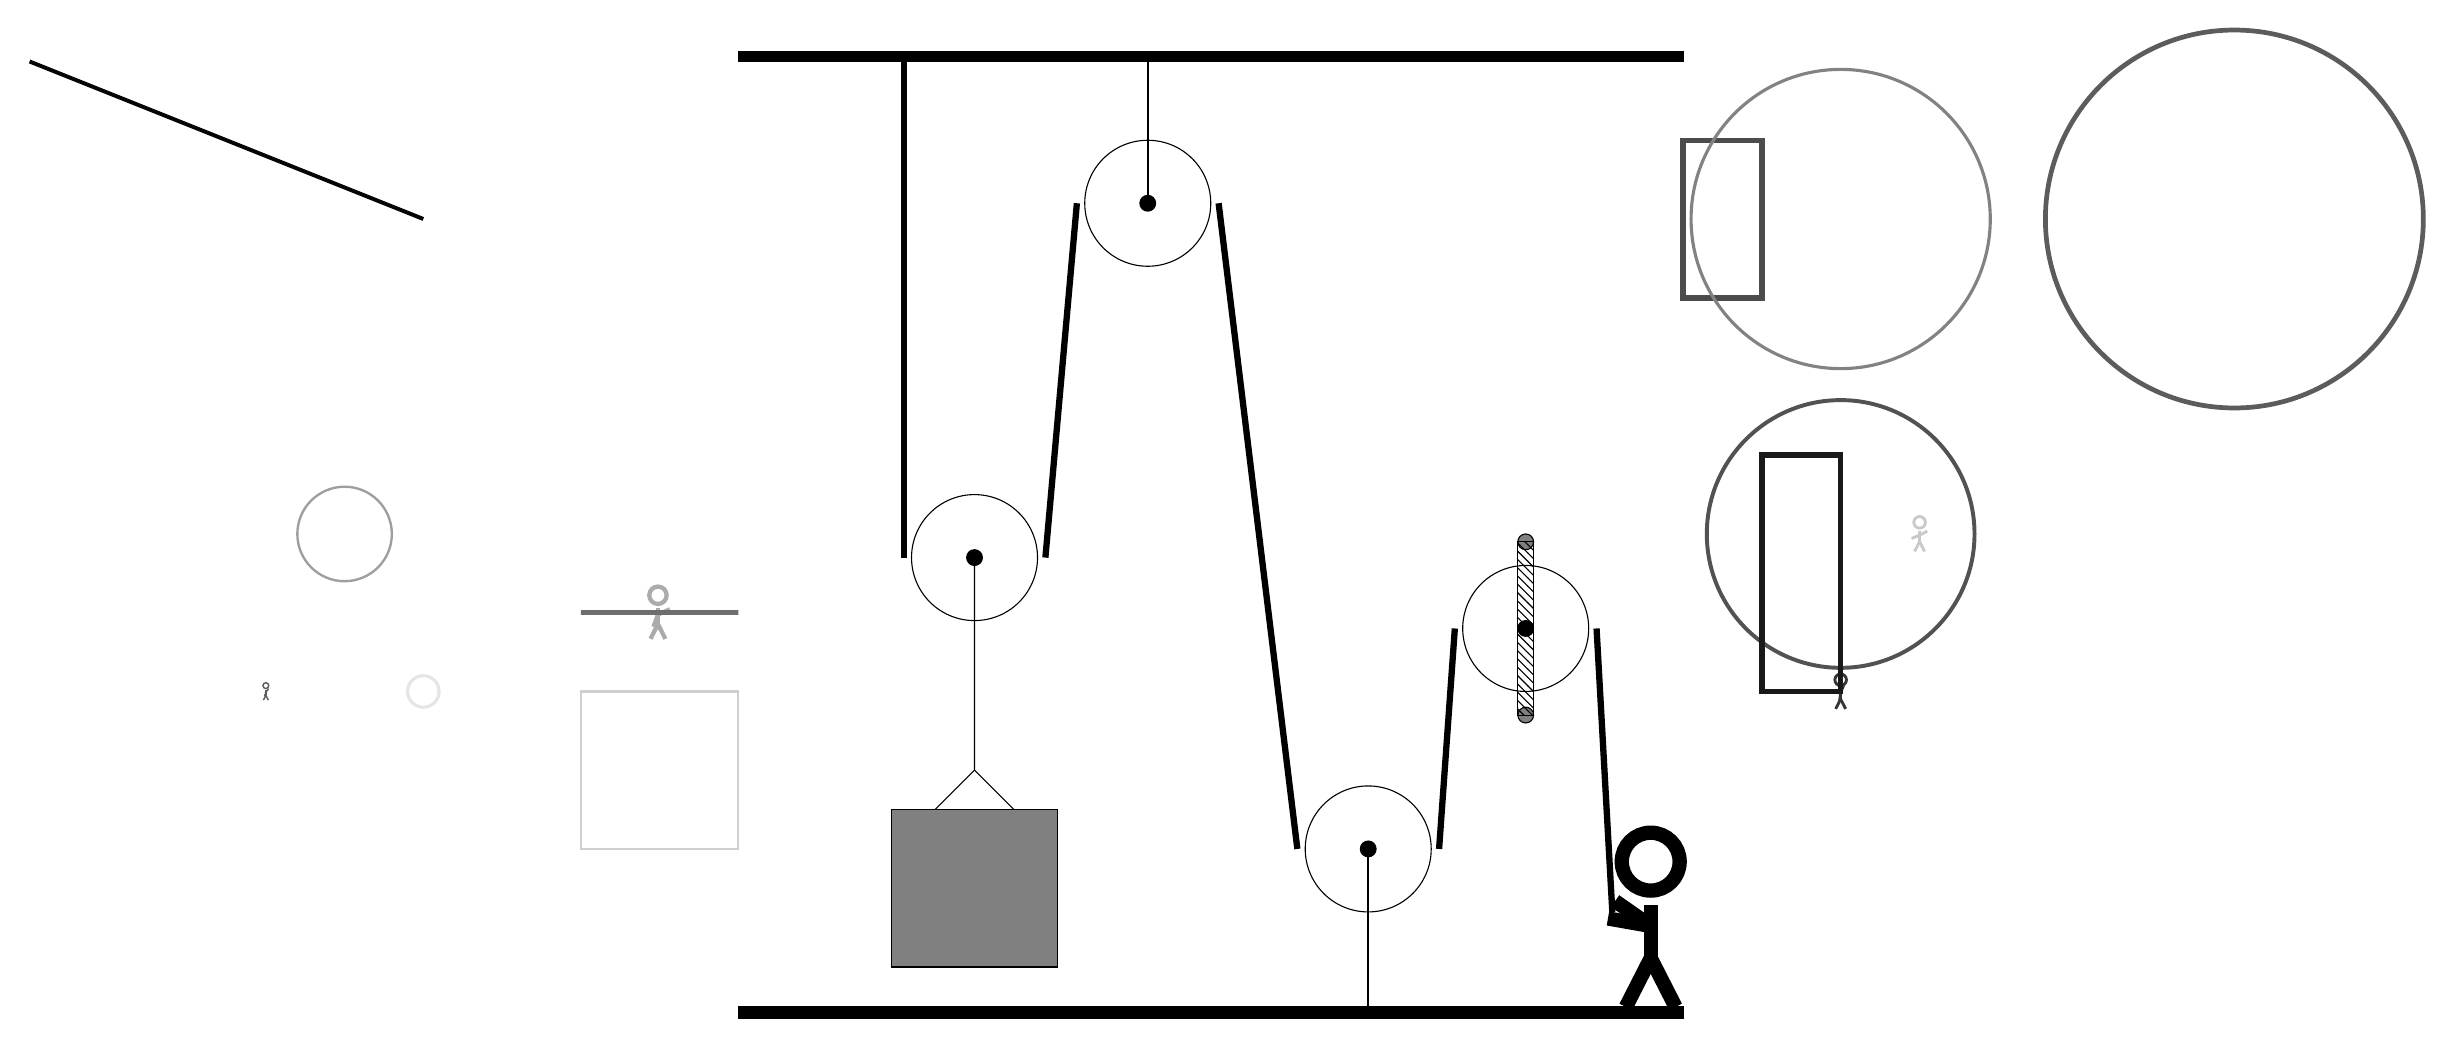
\begin{tikzpicture}
			%%%%% START %%%%%
			
			\draw[fill=black] (-2, 9) rectangle (10, 9.125);
			
			\draw (1, 2.7) circle (0.8);
			\draw[fill=black] (1, 2.7) circle (0.1);
			
			\draw (3.2, 7.2) circle (0.8);
			\draw[fill=black] (3.2, 7.2) circle (0.1);
			\draw[thick] (3.2, 7.2) -- (3.2, 9);
			
			\draw (6, -1) circle (0.8);
			\draw[fill=black] (6, -1) circle (0.1);
			\draw[thick] (6, -1) -- (6, -3);
			
			\node[line width=0.7mm, color=black!79] at (12, 1) {\Strichmaxerl[2][83][68]};
			
			\node[line width=0.3mm, color=black!64] at (-8, 1) {\Strichmaxerl[1][73][50]};
			\draw[line width=0.7mm, color=black!70] (10, 6) rectangle (11, 8);
			\draw [line width=0.6mm, color=black!64](17, 7) circle (2.4);
			\draw [line width=0.3mm, color=black!38](-7, 3) circle (0.6);
			
			\draw[line width=0.5mm, color=black!98](-6, 7) -- (-11, 9);
			\draw[line width=0.3mm, color=black!19] (-4, -1) rectangle (-2, 1);
			\draw [line width=0.4mm, color=black!49](12, 7) circle (1.9);
			\node[line width=0.3mm, color=black!21] at (13, 3) {\Strichmaxerl[2][22][28]};
			
			\node[line width=0.7mm, color=black!33] at (-3, 2) {\Strichmaxerl[3][70][24]};
			\draw[line width=0.6mm, color=black!57] (-4, 2) rectangle (-2, 2);
			\draw [line width=0.5mm, color=black!68](12, 3) circle (1.7);
			\draw[line width=0.7mm, color=black!90] (12, 4) rectangle (11, 1);
			\draw [line width=0.4mm, color=black!10](-6, 1) circle (0.2);
			
			\draw[fill=white](8, 1.8) circle (0.8);
			\draw[fill=black] (8, 1.8) circle (0.1);
			\draw[fill=black!50] (8, 2.9) circle (0.1);
			\draw[fill=black!50] (8, 0.7) circle (0.1);
			\draw[pattern=north west lines, pattern color=black] (7.9, 2.9) rectangle (8.1, 0.7);
			
			\draw (1, 2.7) -- (1, 0) -- (0.5, -0.5);
			\draw (1, 0) -- (1.5, -0.5);
			\draw[fill=black!50] (-0.05, -0.5) rectangle (2.05, -2.5);
			
			\draw[line width=0.8mm] (0.1, 9) -- (0.1, 2.7);
			\centerarc[line width=0.8mm](1, 2.7)(180:360:0.9);
			\draw[line width=0.8mm](1.9, 2.7) -- (2.3, 7.2);
			\centerarc[line width=0.8mm](3.2, 7.2)(0:180:0.9);
			\draw[line width=0.8mm](4.1, 7.2) -- (5.1, -1);
			\centerarc[line width=0.8mm](6, -1)(180:360:0.9);
			\draw[line width=0.8mm](6.9, -1) -- (7.1, 1.8);
			\centerarc[line width=0.8mm](8, 1.8)(0:180:0.9);
			\draw[line width=0.8mm](8.9, 1.8) -- (9.1, -1.8);
			
			\node at (9.5, -1.9) {\Strichmaxerl[10][-35][170]};
			
			\draw[fill=black] (-2, -3) rectangle (10, -3.15);
			
			%%%%% END %%%%%
		\end{tikzpicture}
	\end{figure}	
\end{document}